\documentclass{beamer}
\usetheme{metropolis}           % Use metropolis theme
\usepackage{graphicx}
\usepackage{hyperref}
\usepackage{booktabs}
\usepackage{caption}
\captionsetup{font=small,labelfont=bf}


\title{Insight Glass: Project Presentation}
\subtitle{Software Engineering  Fundamentals, CIE 460}
\author{Aser Osama 202101266 \and Aya Sherif 202100642 \\ \and Gehan Sherif 201902069 \and Omar Ayman 202100443}


\begin{document}

\frame{\titlepage}

\section{Project Scope and Requirements}
\begin{frame}{Project Scope}
    \begin{itemize}
        \item Develop a one of a kind in Egypt web app for professionals.
        \item Help professionals from different disciplines start their careers at companies
        where they can thrive.
        \item Provide a platform for companies to find the best candidates for their job. 
    \end{itemize}
\end{frame}


\subsection{Functional Requirements}
\begin{frame}{Functional Requirements}
    \begin{itemize}
        \item User Registration and Authentication
        \begin{itemize}
            \item Create accounts with email, username, and password.
            \item Email OTP authentication for security.
        \end{itemize}
        \item Profile Management
        \begin{itemize}
            \item Maintain personal profiles with skills, experience, and education.
            \item Upload and manage resumes and documents.
        \end{itemize}
    \end{itemize}
\end{frame}

\begin{frame}{Functional Requirements (cont.)}
    \begin{itemize}
        \item Advanced Company \& Job Search Filters
        \begin{itemize}
            \item Search jobs by keyword, location, industry, or company.
            \item Filter jobs by salary, type, and experience level.
        \end{itemize}
        \item Comprehensive Company Profiles
        \begin{itemize}
            \item Access detailed company profiles with key details.
            \item View employee testimonials for workplace insights.
        \end{itemize}
    \end{itemize}
\end{frame}

\begin{frame}{Functional Requirements (cont.)}
    \begin{itemize}
        \item Transparent Job Listings
        \begin{itemize}
            \item Access detailed job listings which include responsibilities and benefits.
            \item Track application status and updates.
            \item Access company reviews and ratings.
        \end{itemize}
        \item Career Advice
        \begin{itemize}
            \item Access articles, tips, and resources for career development.
            \item Participate in forums and Q\&A sections.
        \end{itemize}
    \end{itemize}
\end{frame}

\begin{frame}{Functional Requirements (cont.)}
    \begin{itemize}
        \item Interactive Discussion Forums
        \begin{itemize}
            \item Join specialized forums for job discussions.
            \item Engage with industry experts and mentors.
        \end{itemize}
        \item Salary Benchmarking Tools
        \begin{itemize}
            \item Access salary data and compare against peers.
            \item View salary visualizations like charts and graphs.
        \end{itemize}
    \end{itemize}
\end{frame}

\begin{frame}{Functional Requirements (cont.)}
    \begin{itemize}
        \item Feedback and Ratings System
        \begin{itemize}
            \item Rate companies and job listings on a standardized scale.
            \item Provide anonymous feedback.
        \end{itemize}
        \item Integration with Social Media Platforms
        \begin{itemize}
            \item Share job listings and profiles on social media.
            \item Link platform profiles with social media accounts.
        \end{itemize}
    \end{itemize}
\end{frame}

\begin{frame}{Functional Requirements (cont.)}
    \begin{itemize}
        \item Interview Preparation Resources
        \begin{itemize}
            \item Share and access interview experiences.
            \item Use guides for various interview types.
        \end{itemize}
        \item Analytics and Insights Dashboard
        \begin{itemize}
            \item Admin access to track user engagement and trends.
            \item Comprehensive data visualization tools.
        \end{itemize}
    \end{itemize}
\end{frame}


\begin{frame}{Non-functional Requirements}
    \begin{itemize}
        \item Security and Privacy (SSL Encryption, Identity Framework, etc.)
        \item Performance (Caching \& Load Balancing)
        \item Scalability (Azure Scalable Web Apps)
        \item Reliability (Constant Monitoring, Logging, Alerts \& Testing)
    \end{itemize}
\end{frame}

\section{Project Design and Architecture}

\begin{frame}{Project Architecture}
We followed a 3-tier architecture with all components hosted as scalable components on Azure.
    \begin{figure}
        \centering
        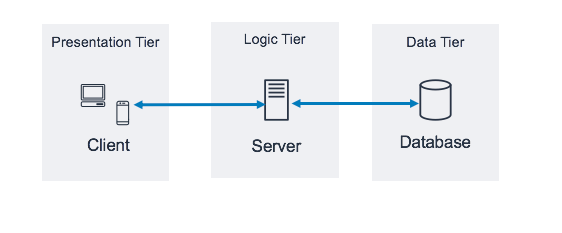
\includegraphics[width=1\textwidth]{Images/Archircture.png}
        \caption{Archircture Diagram}
    \end{figure}
\end{frame}

\begin{frame}{Project Archircture (cont.)}
    \begin{itemize}
        \item Frontend \& Backend: React.js hosted on Azure Web Apps as a containerized scalable app.
        \item Database: Azure MySQL Database for storing user, job, and company data.
        \item Devops: CI/CD Pipeline using GitHub Actions for automated deployment.
    \end{itemize}
\end{frame}

\begin{frame}{Design Patterns and OO Principles}
    \textbf{Design Patterns:}
    \begin{itemize}
        \item Singleton Pattern for React Context: Helps us persist user state across components.
        \item Factory Pattern for the database connection: Make the most out of Entity Framework caching and 
        performance by following it's best practices. 
        \item Strategy Pattern
        \item Dependency Injection in Web API controllers: We inject services and database context to controllers.
        \item Dependency Injection in React: We build our components to be reusable.
    \end{itemize}
\end{frame}

\begin{frame}{Design Patterns and OO Principles (cont.)}
\textbf{SOLID Principles}
    \begin{itemize}
        \item Single Responsibility Principle: Each of the controllers is responsible for a single model.
        \item Open/Closed Principle: API controllers are easily extendable.
        \item Interface Segregation Principle: We can use partial classes in C\#.
        \item Dependency Inversion Principle: All communication was top down.
    \end{itemize}
\end{frame}

\section{Devops}
\begin{frame}{Scrum Implementation}
    \begin{itemize}
        \item We used GitHub Projects to manage our Scrum workflow.
        \item We help bi-weekly stand-ups that were changed to bi-daily in later stages.
        \item We had multiple Sprint Reviews and Retrospectives
    \end{itemize}
\end{frame}
\begin{frame}{Scrum Implementation (cont.)}
    \begin{figure}
        \centering
        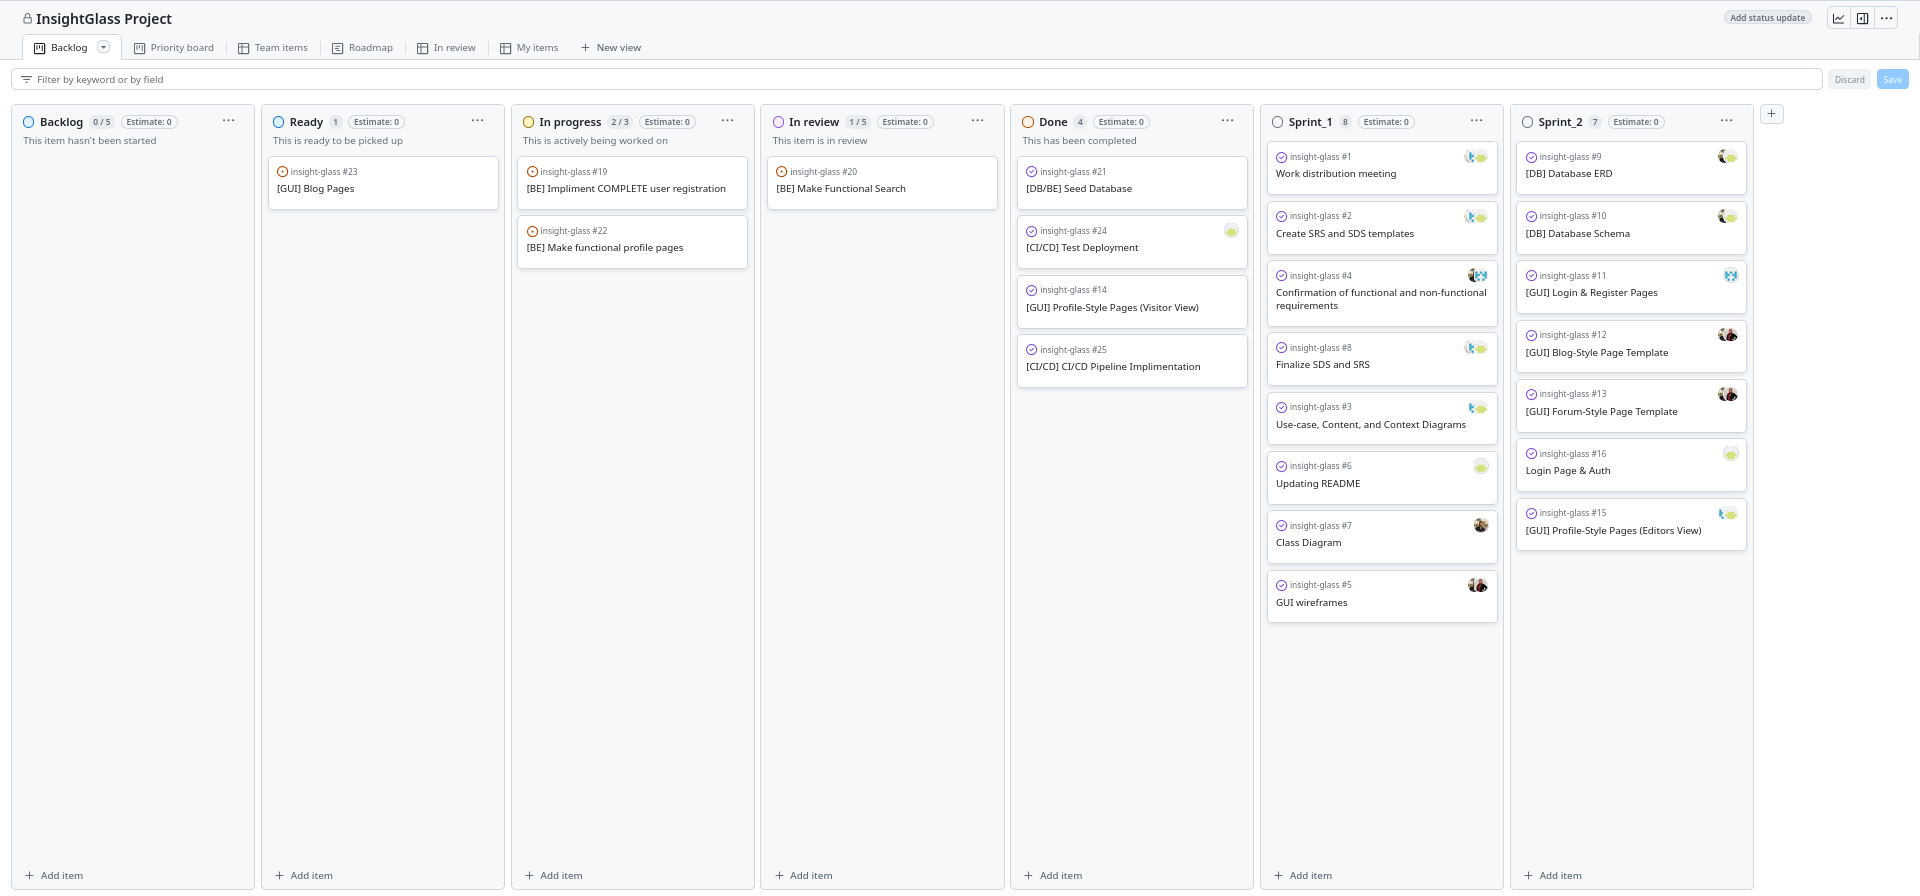
\includegraphics[width=1\textwidth]{Images/ScrumBoard.png}
        \caption{Scrum Board}
    \end{figure}
\end{frame}

\begin{frame}{CI/CD Pipeline}
    \begin{enumerate}
        \item Version Control using Git and GitHub
        \item Automated Unit Testing using XUnit, Moq, \& Entity Framework Core - InMemory, 
        \item Automated Integration Testing using Selenium (in progress)
        \item Continuous Integration using GitHub Actions to Azure Container Registry
        \item Continuous Deployment to Azure Web App
    \end{enumerate}

\end{frame}
\begin{frame}{CI/CD Pipeline}
    \begin{figure}
        \centering
        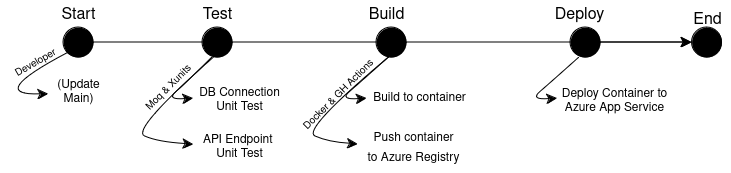
\includegraphics[width=1\textwidth]{Images/Devops.png}
        \caption{CI/CD Pipeline}
    \end{figure}
\end{frame}


\section{Reflections}

\subsection{Challenges Encountered}
\begin{frame}{Challenges Encountered}
    \begin{itemize}
        \item \textbf{Technical Challenges}
        \begin{itemize}
            \item Learning React and .NET
            \item Lack of resources (using latest releases of .NET and React.)
            \item Lack of mentorship.
            \item Time constraints due to semester schedule and holidays.
        \end{itemize}
    \end{itemize}
\end{frame}

\subsection{What Went Wrong}
\begin{frame}{What Went Wrong}
    \begin{itemize}
        \item \textbf{Time Management}
        \begin{itemize}
            \item Overly optimistic estimates.
            \item Delayed starts and rushed efforts due to clashing deadlines.
        \end{itemize}
        \item \textbf{Task Breakdown}
        \begin{itemize}
            \item Ineffective task division.
            \item Underestimated complexity of React and .NET integration.
        \end{itemize}
        \item \textbf{Documentation}
        \begin{itemize}
            \item Lack of internal documentation (Common flaw of Scrum/Agile development).
            \item Inconsistent coding standards initially.
        \end{itemize}
    \end{itemize}
\end{frame}

\subsection{What Went Well}
\begin{frame}{What Went Well}
    \begin{itemize}
        \item \textbf{Team Collaboration}
        \begin{itemize}
            \item Effective collaboration and communication.
            \item Peer support and knowledge sharing.
        \end{itemize}
        \item \textbf{Adaptability}
        \begin{itemize}
            \item Quickly learned and applied new technologies.
            \item Improved technical skills and confidence.
        \end{itemize}
    \end{itemize}
\end{frame}

\subsection{How to Improve}
\begin{frame}{How to Improve}
    \begin{itemize}
        \item \textbf{Start Earlier}
        \begin{itemize}
            \item Begin planning and development sooner.
        \end{itemize}
        \item \textbf{Seek Mentorship}
        \begin{itemize}
            \item Engage mentors early for feedback.
        \end{itemize}
        \item \textbf{Better Time Management}
        \begin{itemize}
            \item Implement realistic time estimates.
            \item Use project management tools effectively.
        \end{itemize}
        \item \textbf{Effective Task Breakdown}
        \begin{itemize}
            \item Break tasks into smaller, manageable units.
            \item Regularly review and adjust task allocations.
        \end{itemize}
    \end{itemize}
\end{frame}

\begin{frame}{How to Improve (cont.)}
    \begin{itemize}
        \item \textbf{Documentation}
        \begin{itemize}
            \item Maintain comprehensive documentation.
        \end{itemize}
        \item \textbf{Continuous Feedback}
        \begin{itemize}
            \item Establish regular check-ins and feedback loops.
        \end{itemize}
    \end{itemize}
\end{frame}

\subsection{Conclusion}
\begin{frame}{Conclusion}
    \begin{itemize}
        \item Significant learning experience.
        \item Developed crucial skills and insights.
        \item Future improvements will enhance project success.
    \end{itemize}
\end{frame}


\section{Discussion}



\begin{frame}{Questions}
    \begin{center}
        \Huge{Questions?}
    \end{center}
\end{frame}

\end{document}
